

\part{Getting started}
\label{part:GettingStarted}

\chapter{Overview}

\section{Introduction}

This part of the book will run the reader through the LedgerSMB using an example
startup company run by Jack: Example Inc, which starts its life as a computer parts
store for the business to business market.

Jack just completed incorporation of Example and is ready to start doing business.
Before starting his operation Jack decides to look for tooling to run his operation
efficiently.

The other chapters in this part of the book show you what steps Jack has to go through
to get LedgerSMB up and running for Example, as well as the steps he has to take to
keep LedgerSMB in good health.

Due to its success Example will grow, posing new challenges to LedgerSMB and we'll show
you how Jack can change the configuration to adapt to his growing business's needs.

It's outside the scope of this part to explain how to install the application. See
Part \ref{part:Configuration} for information on installation. \charef{cha:CompanyCreation}
starts when the software has been installed yet nothing more has been done.

\section{LedgerSMB, because...}

Jack finds several tools which suit his requirements to some extent or another.
After evaluation of his options he decides to use LedgerSMB for the following reasons:

\begin{itemize}
\item Centralized data storage
\item Actively developed
\item Development team with security focus
\item Access to the application requires only a web browser
\item Integrated sales, shipping, invoicing, purchasing and accounting
\item Open source solution, so no vendor lock in
\item @@@ others?
\end{itemize}

He'll be running LedgerSMB using the domain he acquired for his business:
\url{http://example.com/}.

\chapter{Creating a company administration}
\label{cha:CompanyCreation}

\section{Using setup.pl}

% some introduction

Please note that while executing the steps described in this section, presentation of
the next screen may take a while after clicking on each button. Some buttons involve
a large amount of processing on the server before the next screen can be presented.

\subsection{Step 1: setup.pl login}

\begin{figure}[h]
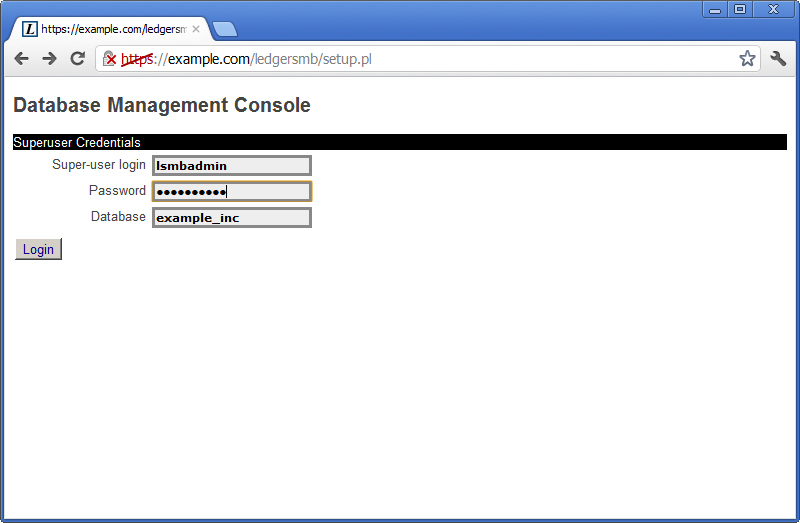
\includegraphics[width=\linewidth]{dmc-create-step1.png}
\caption{setup.pl login screen}
\end{figure}
\label{fig:setup-step1}

\subsection{Step 2: Company creation}

\begin{figure}[h]
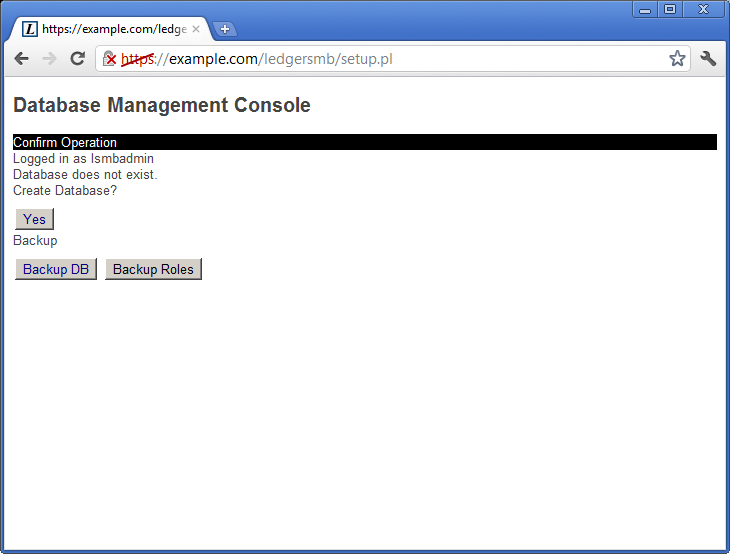
\includegraphics[width=\linewidth]{dmc-create-step2.png}
\caption{setup.pl company creation screen}
\end{figure}
\label{fig:setup-step2}


\subsection{Step 3: Selection of a Chart of Accounts}

\begin{figure}[h]
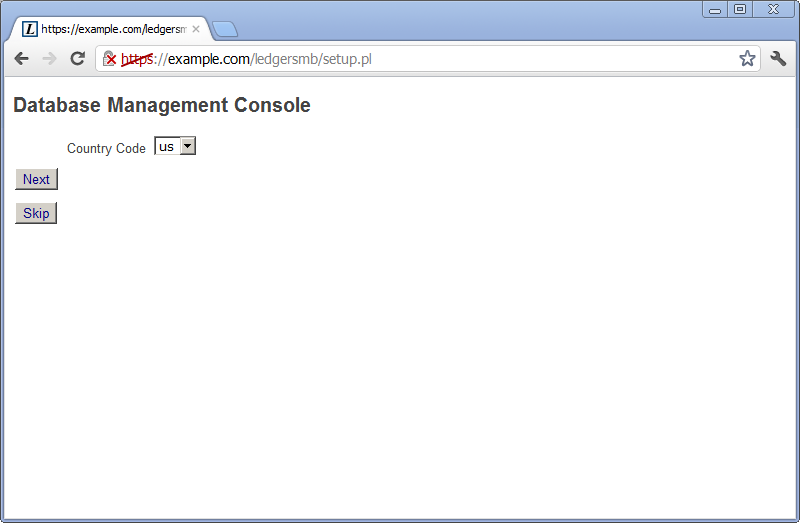
\includegraphics[width=\linewidth]{dmc-create-step3.png}
\caption{Chart of accounts - Country selection}
\end{figure}
\label{fig:setup-step3}

\begin{figure}[h]
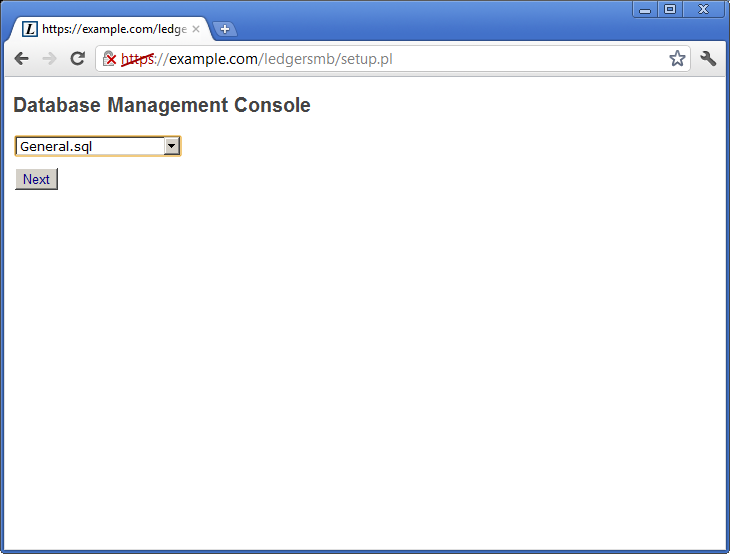
\includegraphics[width=\linewidth]{dmc-create-step4.png}
\caption{Chart of accounts - Chart selection}
\end{figure}
\label{fig:setup-step4}


\subsection{Step 4: First user}

\begin{figure}[h]
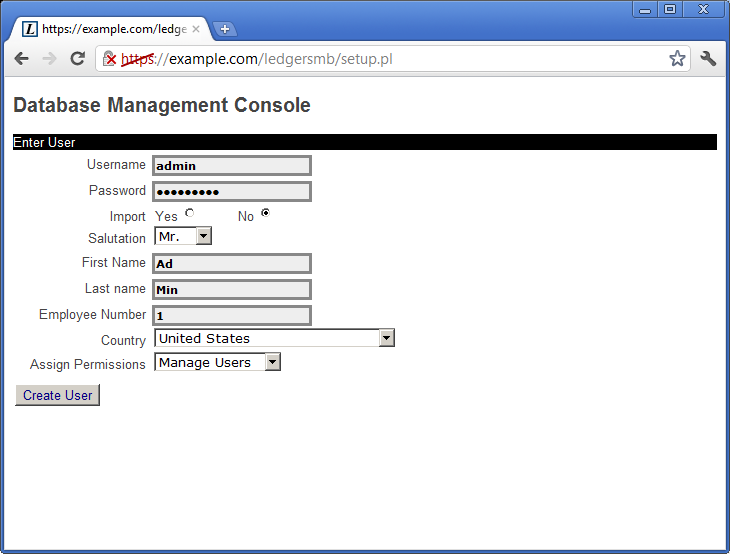
\includegraphics[width=\linewidth]{dmc-create-step5.png}
\caption{setup.pl initial user creation screen}
\end{figure}
\label{fig:setup-step5}

\begin{figure}[h]
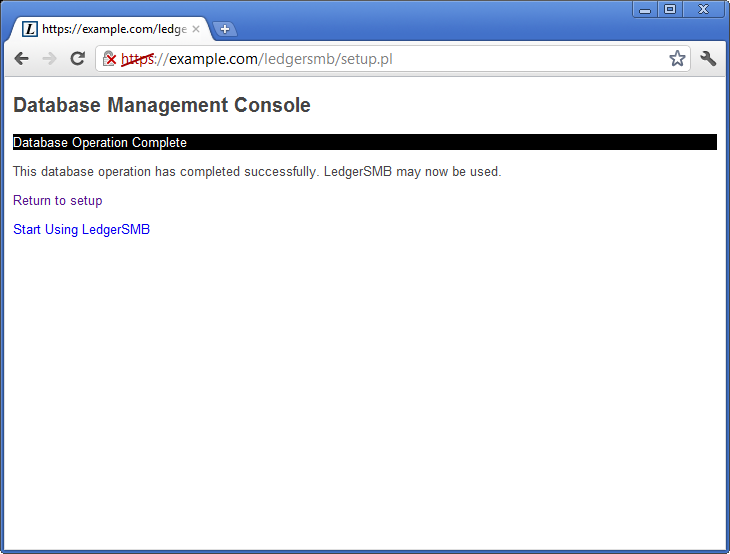
\includegraphics[width=\linewidth]{dmc-create-step6.png}
\caption{setup.pl succesfull completion screen}
\end{figure}
\label{fig:setup-step6}


\chapter{The first login}

\section{Introduction}

Upon first login it's best to set up the system configuration parameters. This
prevents running into errors due to partial configuration later on.

This chapter assumes you've loaded a chart of accounts in \charef{cha:CompanyCreation}.

\section{Steps to the first login}

\subsection{Login screen}

\subsection{Selecting a password}

\subsection{Subsequent logins}


\section{Setting up the system defaults}

This section can only be completely filled out when a chart of accounts has been loaded.

A more elaborate description of the parameters in this section is provided in subsection
\ref{subsec:Defaults}. However, when setting up a new company, it's probably good enough
to fill out these parameters (and thus skip the rest):

\begin{itemize}
\item Business number (e.g. Chamber of commerce number) [12345]
\item Default language [English]
\item Default accounts (Inventory, Expense, Income) [@@@]
\item Foreign exchange result accounts (Foreign exchange gain/loss) [@@@]
\item Default country [US]
\item Templates directory [demo]
\item Currencies [USD:CAD]
\item Default Email From [info@example.com]
\item Company Name [Example Inc.]
\item Company Address [215 Example street - Whereitsat]
\item Company Phone [555 836 22 55]
\item Company Fax (optional) [N/A]
\end{itemize}

Jack enters the values mentioned between the square brackets in the list above. 
He used one of the charts of accounts (CoA) that came with LedgerSMB and therefore
checks the Taxes page in the System menu to see if the percentages that were delivered
with it are still current.

\section{Setting up a bank account or credit card}

As part of the start up activities of his company, Jack comes to an agreement with the
bank for three products:

\begin{itemize}
\item A current account with number C54769
\item Deposit account with number D54990
\item Credit card with a number ending with .7734
\end{itemize}

Most accounting systems - LedgerSMB included - use separate GL accounts to represent
each bank account. This allows easy reconciliation of the ending balance on the bank
account with the balance in the books.

Knowing this, Jack looks up the example bank account from his preconfigured US chart of
accounts using the System $\rightarrow$ Chart of Accounts $\rightarrow$ List Accounts menu as
shown in % ###figref:

\begin{itemize}
\item Renames the original item into ``Bank account C54769''
\end{itemize}


\chapter{Building up stock}

\chapter{Ramping up to the first sale}

% sending out a quote followed by a sales order

\chapter{Shipping sales}

\chapter{Invoicing}

\chapter{Collecting sales invoice payments}

\section{Customer payments}

\section{Customer payment mismatch}

% choosing between pardonning and registering underpayment

% large ones, as in partial payments or largish under/over payments

% pardonning small mismatches


\chapter{Paying vendor invoices}

% handling vendors who match amounts to exact invoices

% handling vendors with running balances

% handling bounced checks: voiding checks to undo payments of vendor invoices
%   relating to bounced checks

\chapter{Monitoring arrears}

% handling interest on arrears

\chapter{Handling sales taxes}

% invoices with taxes included

% invoices with explicit tax amounts

% 

\chapter{Branching out: services}

% including creation / assignment to different accounts


\chapter{Recording service hours}

\chapter{Customer approval on service hours}

\chapter{Invoicing services}

\chapter{Branching out II: service subscriptions}


